    \chapter{Methodology}
       \section{SOFTWARE DEVELOPMENT APPROACH}
        Prototyping model is a type of software develpoment model. It is an iterative approach where a basic prototype is constructed to gain a better understanding of the project. This prototype is typically incomplete or lacking many components. The model is then refined based on feedback and system is reconstructed iteratively until desired conditions are met.
         \begin{figure}[hbt!]
            \centering
                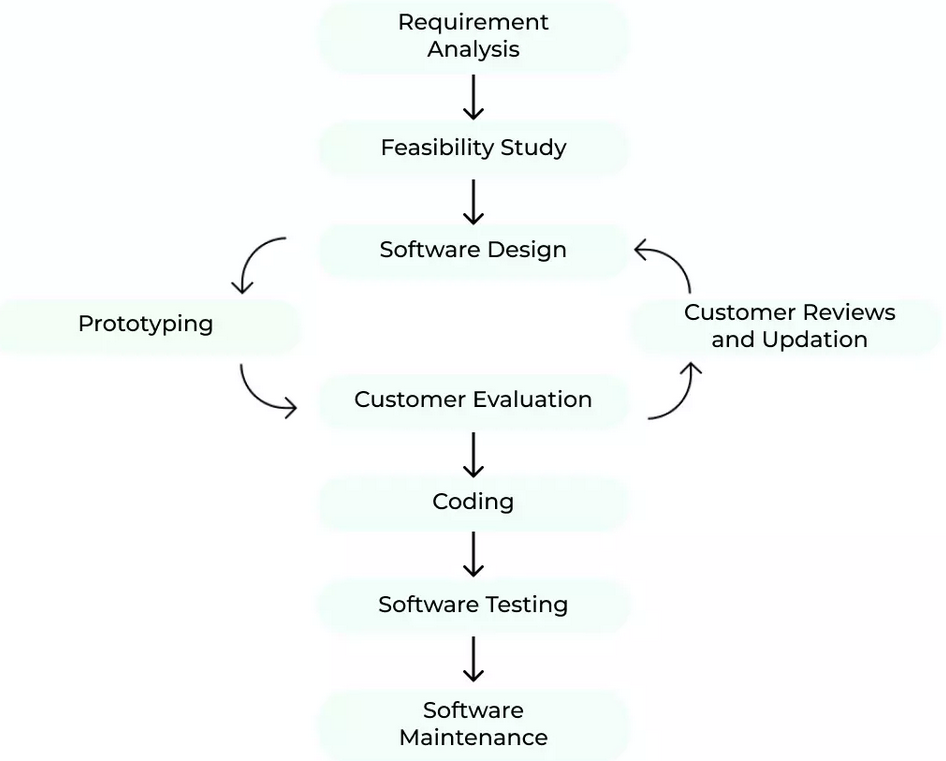
\includegraphics[width=0.75\textwidth]{./img/prototype model.png}
                \caption{Prototype Model for Software Development}
        \end{figure}
        \section{DATA COLLECTION}
        We have found many datasets on the internet from popular platforms like kaggle, github. For this project we will be using the datasets provided by ondyari/ FaceForensics \url{https://github.com/ondyari/FaceForensics}.\\
            For POS tagging, the data from NELRALEC [10] The following table shows the amount
            of data collected from different sources and their usage in our project;

    
        \section{Implementation}
        Deepfake images are structured and classified into fake and real face. The data set generated is splited into training set and test set. The training set is then fed into a Deep learning model (ResNet Architecture). This model is tested whether it can identify/detect the fake face using the test data.

        \vspace{0.5in}
        \begin{figure}[hbt!]
            \centering
                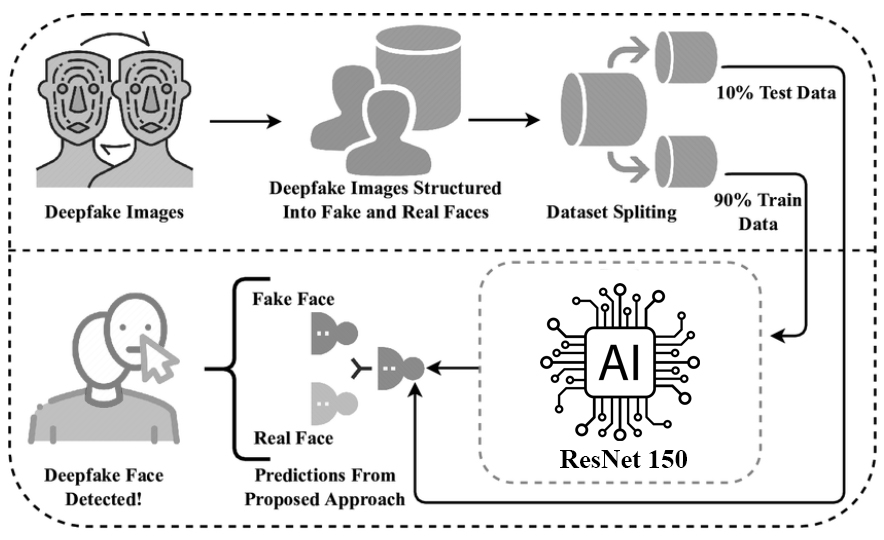
\includegraphics[width=1\textwidth]{./img/implementation.jpg}
                \caption{Methodological Architecture of Our Proposed System}
        \end{figure}

        \subsection*{ResNet}
        ResNet architecture introduced the concept called Residual Blocks. In this network, we use a technique called skip connections. The skip connection connects activations of a  layer to further layers by skipping some layers in between. This forms a residual block. Resnets are made by stacking these residual blocks together. 
        The approach behind this network is instead of layers learning the underlying mapping, we allow the network to fit the residual mapping. So, instead of say H(x), initial mapping, let the network fit,
        \center{F(x) := H(x) - x 
            which gives H(x) := F(x) + x}

        \begin{figure}[hbt!]
            \centering
                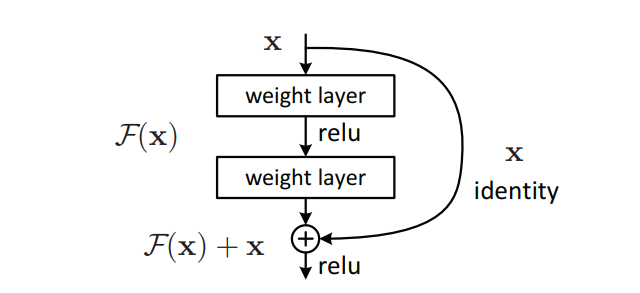
\includegraphics[width=1\textwidth]{./img/ResNet.PNG}
                \caption{Working of ResNet}
        \end{figure}

        \begin{figure}[hbt!]
            \centering
                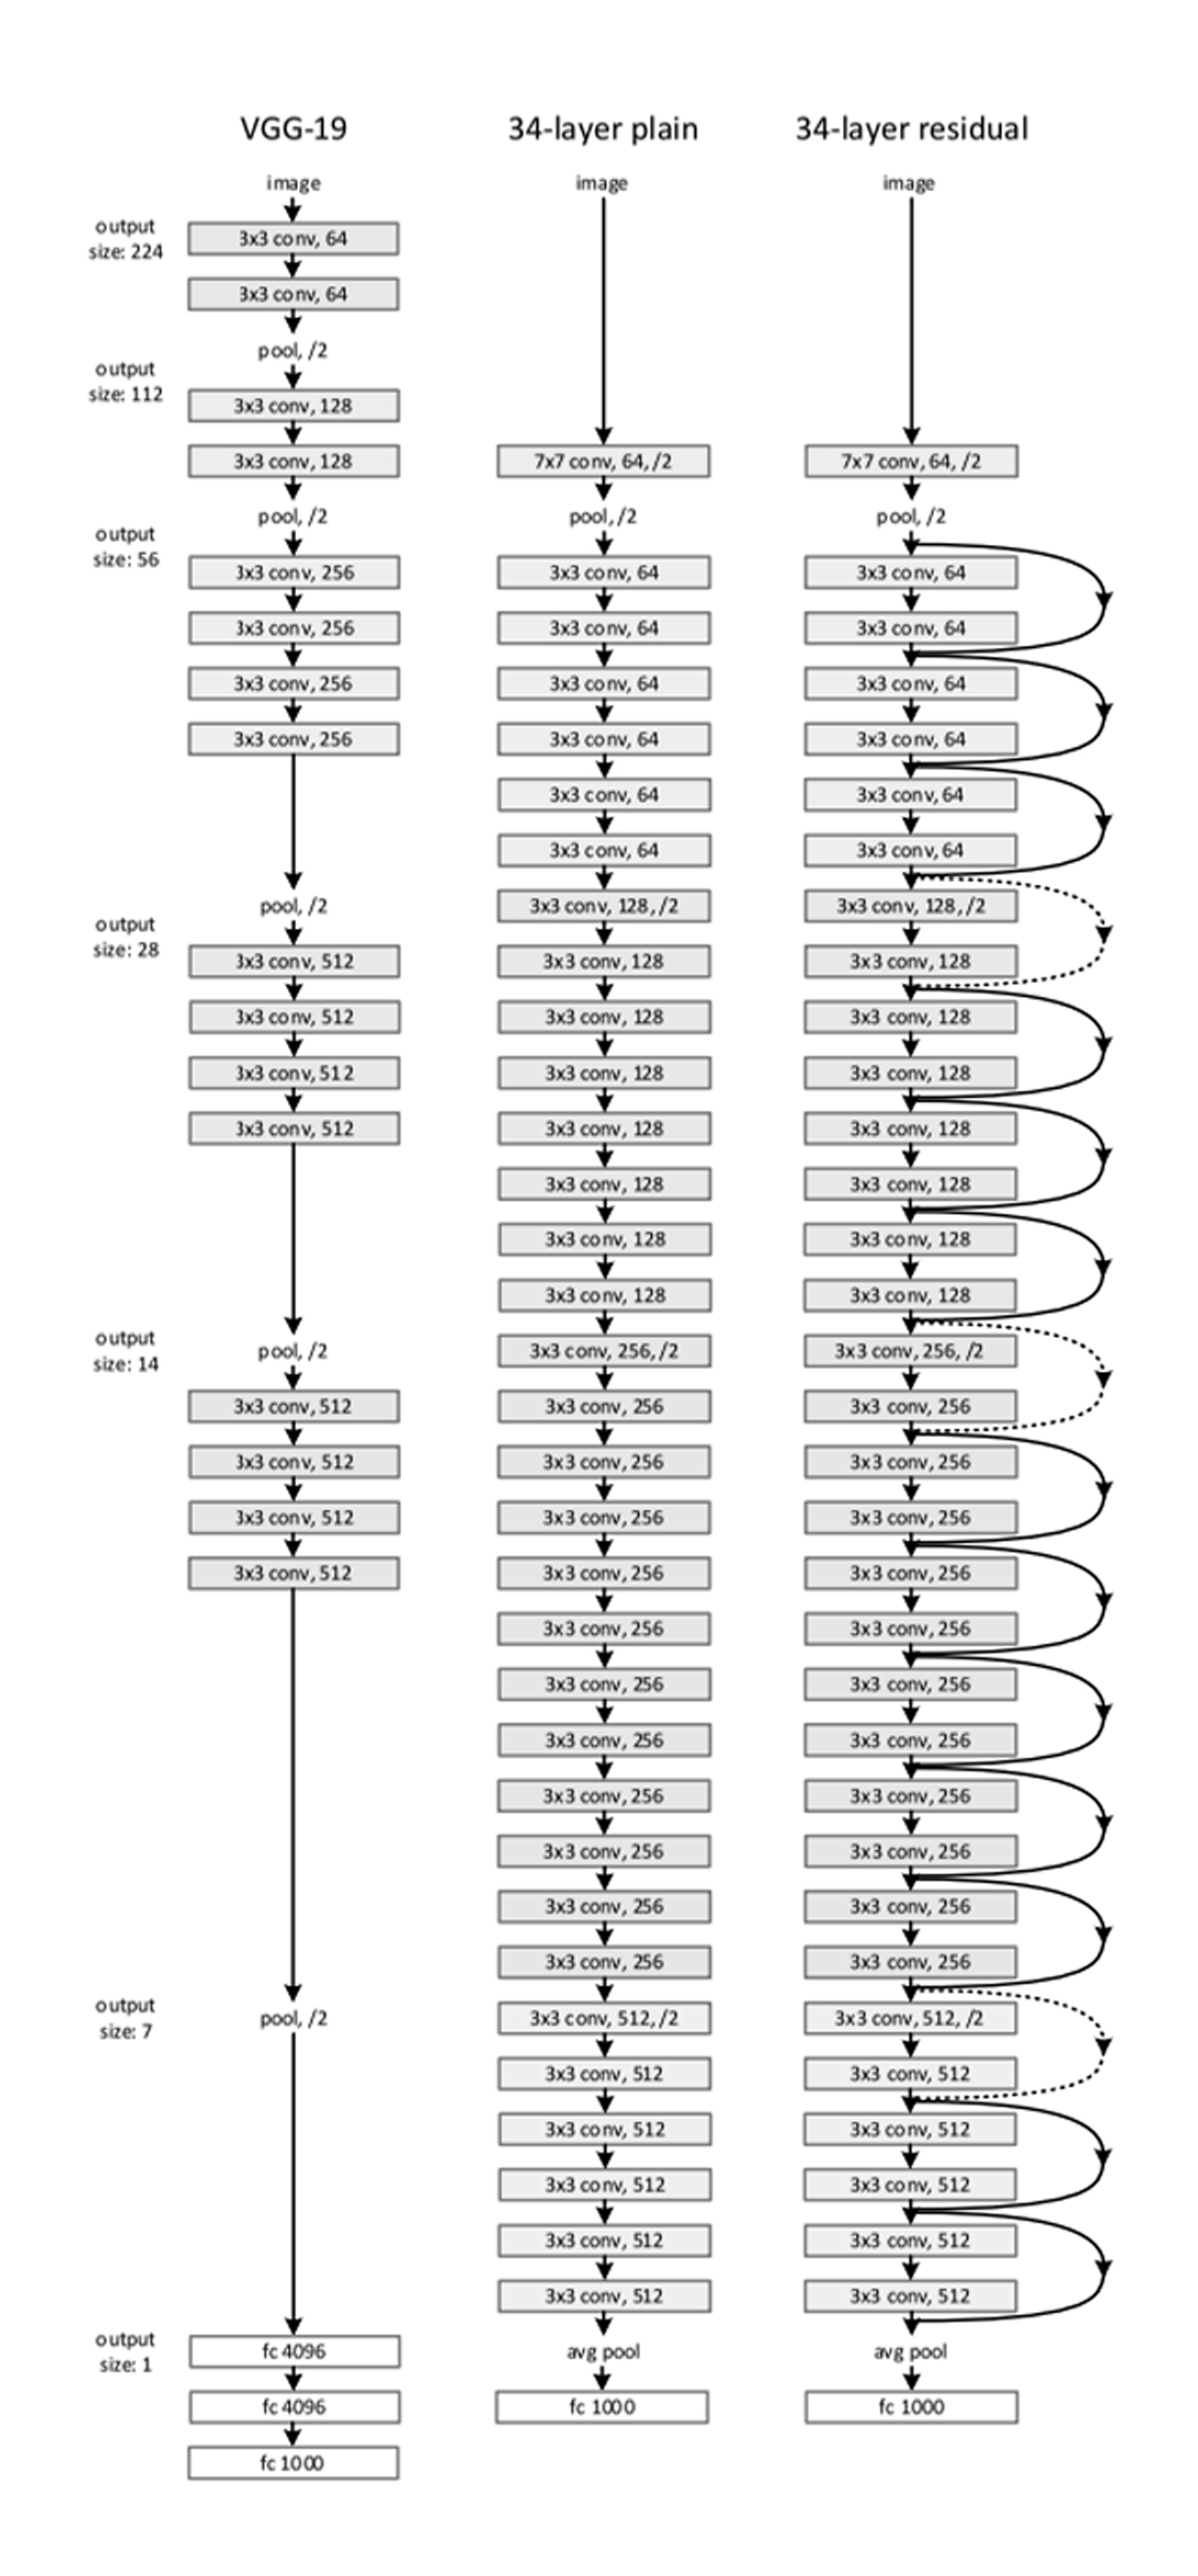
\includegraphics[height=1.4\textwidth]{./img/ResNetArc.jpg}
                \caption{ResNet Architecture}
        \end{figure}
% 10Table 6.1 Data Sources with numbers\\

%     \begin{table}[h]
%         \caption{Data Sources with numbers}
%         \begin{tabular}{|c|c|c|}
%             \hline
%             \textbf{Source} & \textbf{Number of Data}  & \textbf{Usage} \\\hline
%             Nepali News Corpus & 14364 Articles  & Vectorization\\\hline
%             Facebook & 5021 Comments & Labeling\\\hline
%             Twitter & 2160 Tweets & Labeling\\\hline
%             Annapurnapost.com & 400 Articles Vectorization, & Labeling\\\hline
%             Nagarik News & 4481Articles & Vectorization\\\hline
%             National News & 7452 Articles & Vectorization\\\hline
%             Bsgnews.com & 1000 Articles & Vectorization, Labeling\\\hline
%             Setopati News & 1090 Articles & Vectorization\\\hline
%             NELRALEC Corpora & 798961 Sentences & POS Tagging\\\hline
%         \end{tabular}
%     \end{table}

%             \subsection{Twitter Tweet Collection}
% We applied for Twitter Developer Account to get API keys to gather data from twitter.
% Tweepy
% [9]
% which is a python tweet API library was used to make API requests and
% model the response in appropriate format. We used some of the queries for the API like;
% ‘brb1954’, ‘hello_sarkar’, ‘thapagk’, ‘nepalitweet’ etc. From these queries the tweets
% were returned which then was tokenized into sentences and modeled finally saving into
% JSON format. JSON format was used because serialization and deserialization of Tweet
% model as easy in JSON format than other formats like; CSV, XLS. The tweet format
% for saving the data is shown in the figure below;

%         \begin{figure}[hbt!]
%             \centering
%              \includegraphics[width=0.5\textwidth]{./img/6.2.jpg}
%                 \caption{Tweet in JSON Format}
%         \end{figure}
%         \begin{figure}[hbt!]
%             \centering
%              \includegraphics[width=00.5\textwidth]{./img/6.3.jpg}
%                 \caption{Tweet tokenization and storing flow chart}
%         \end{figure}
% In this way JSON formatted tweets is passed into Data Labeling System (Section 6.6)
% and stored in MySQL for easy access from database rather than flat file.
%             \section{DATA PREPARATION}
% After the data has been collected, it was processed to make into correct format so that
% the neural networks can understand both the inputs and outputs. The block diagram
% (figure 6.2) shows the data preparation steps of the project.
%         \begin{figure}[hbt!]
%             \centering
%                 \includegraphics[width=0.9\textwidth]{./img/6.4.jpg}
%                 \caption{Data Preparation Block Diagram}
%         \end{figure}

%                 \subsection{Tokenization}
% The unlabeled and unprepared data is fed into the tokenization engine. There are two
% types of tokenization; one sentence level tokenization and another word level
% tokenization. Following example shows both the sentence level tokenization as well as
% world level tokenization.
%         \begin{figure}[hbt!]
%             \centering
%                 \includegraphics[width=0.5\textwidth]{./img/6.5.jpg}
%                 \caption{Tokenization }
%         \end{figure}
%             \subsection{Stop Words Removal}
% The tokenized Nepali words will now be preprocessed to remove stop words such as;
% छ, हो etc. which has no meaning or participation in sentiment analysis. This stop word
% removed tokenized data will now be fed into stemming algorithm.
%         \begin{figure}[hbt!]
%             \centering
%                 \includegraphics[width=0.5\textwidth]{./img/6.6.jpg}
%                 \caption{Stop Words Removal Process}
%         \end{figure}                    \subsection{Stemming}
% We will use snowball
% [11]
% rule-based stemming algorithm for removing some of the
% stems of the Nepali language such as; को, का, कक etc.
%         \begin{figure}[hbt!]
%             \centering
%                 \includegraphics[width=0.5\textwidth]{./img/6.7.jpg}
%                 \caption{Stemming Process}
%         \end{figure}
%             \subsection{Word2Vec}
% As neural networks require numbers as the inputs. The tokenized words need to be
% converted into feature vectors i.e. list of numbers. Not any random list of number but
% the related numbers. There must be a correlation between two tokenized words i.e. two
% vectors must be correlated with each other. Example: In English language, king and
% boy are more related than queen and girl so king and boy’s vector representation should
% be near to each other than other words. Word2Vec
% [12]
% converts those sentences into
% context linked vector representation as the name suggests.
%             \subsection{Labeling System}
% From the unprocessed data, we need to manually label the data points. For manually
% labeling the data points we created a system from PHP programming language; reading
% the data points from MySQL database and then let the user choose between positive or
% negative sentiment and record it in database all hosted in internet for easy access. The
% data labeling system is described in detail in section 6.6 of this report.
%             \subsection{POS Tagging}
% POS tagging is a piece of software that assigns parts of speech to each word and some
% other token. From the word vectors and their respective POS (Parts of Speech) tags
% need to be placed by the system. POS tagging gives more insight to the data making
% neural network little bit easier to classify sentiment data. Some of the list of POS tags
% can be seen in the table below;
%     \begin{table}[hbt!]
%         \centering
%         \caption{Some of the POS Tags from NELRALEC Tagset}
%        \begin{tabular}{|p{3cm}|p{5cm}|p{3cm}|}
%             \hline
%             \textbf{POS Tags} & \textbf{Description} & \textbf{Example} \\
%             \hline
%             NN & Common Noun &  के,टोके,टाकलम \\
%             \hline
%             NP & Proper Noun & राम, युबराज  \\
%             \hline
%             JM & Masculine Adjective & मोटो, पातलो \\
%             \hline
%             JF & Feminine Adjective  & दुब्ली,मोटी  \\
%             \hline
%              VI & Infinite Verb & गर्ुु,र्गर्ुु \\
%             \hline
%               ... & ... & ... \\
%             \hline
%         \end{tabular}
%     \end{table}

% The following figure below shows the POS Tagging system with example in Nepali
% Language:
%         \begin{figure}[hbt!]
%             \centering
%                 \includegraphics[width=0.5\textwidth]{./img/6.8.jpg}
%                 \caption{POS Tagging System example taken from ANN Based POS Tagging for Nepali Text}
%         \end{figure}
%             \subsection{One Hot Encoder}
% One Hot encoding or Binarization is the process of converting the labeled data into
% binary labels. The encoding scheme of our project is shown in the table below;
% Table 6.3 One Hot Encoding4
%         \begin{table}[hbt!]
%             \centering
%             \caption{One Hot Encoding}
%             \begin{tabular}{|c|c|}
%                 \hline
%                 \textbf{Labels}   & \textbf{Binarization} \\ \hline
%                 Positive & {[}1,0{]}   \\ \hline
%                 Negative & {[}0,1{]}   \\ \hline
%             \end{tabular}
%         \end{table}

%         \section{TRAINING}
% After data has been prepared the data is fed into various models described in Section
% 6.5.3 to 6.5.6 in this report. Various models’ evaluation was carried out after training
% the model. The data will be fed into the training system or neural network as shown in
% the figure below;
%         \begin{figure}[hbt!]
%             \centering
%                 \includegraphics[width=0.5\textwidth]{./img/6.9.png}
%                 \caption{Basic Machine Learning Training Process}
%         \end{figure}
%         \section{ALGORITHMS AND MODELS}
% As above mentioned, various algorithms and models were developed for building the
% sentiment classification engine. Following topics describes all the algorithms and
% models used in the project in detail;
%             \subsection{Tokenization Algorithm}
% There is the use of Regular Expressions also known as RegEx for splitting the
% documents into tokens. There are two types of tokenization into play namely; sentence
% level tokenization and word level tokenization. Since, Nepali language sentences are
% separated with special characters like purnabiram (।) or question marks (?) it is easy to
% split them into sentences with the use of RegEx. The algorithm for sentence level
% tokenization is given below;
% Sentence Level Tokenization Algorithm
%                 \begin{enumerate}
%                     \item Start
%                     \item Input Nepali Sentences
%                     \item RegEx Split Sentences /(?<=[।?!]) +/
%                     \item Output split chunks of Nepali Sentences
%                     \item End
%                 \end{enumerate}
% In languages that have words separated by blank spaces, the token boundary for word-
% level tokenization is the blank/white space. Nepali is one such language so word-level
% tokenization in Nepali can be achieved by stripping tokens at those white spaces.
% However, it is not as simple as it looks, especially when dealing with punctuations.
% Some punctuation is easy to handle. We first need to replace punctuations with white
% spaces. Similarly hyphen (-) which is used in linking word pairs: opposite, analogy or
% similar, together. In this case hyphen is considered as the part of token itself. However,
% hyphen might occur independently in such cases we need to attach the words to make
% it a single token. Similarly, colon (:) and period (.) can be considered as the part of
% token itself. The algorithm for word level tokenization can be seen below:
%                 \textit{Word Level Tokenization Algorithm}
%                 \begin{enumerate}
%                     \item Start
%                     \item Input Sentence
%                     \item Replace punctuations with white spaces
%                     \item Make all words with (:, ., -) symbols a single token
%                     \item Split the formed sentences according to white spaces
%                     \item Output the tokenized sentences
%                     \item End
%                 \end{enumerate}
%                 \subsection{Stemming Algorithm}
% The stemming algorithm was used in our project to reduce the redundancy imposed by
% various words coming from the same stems meaning similar definition for this already
% implemented algorithm in snowball was used. Snowball is a small string processing
% language which was designed for creating stemming algorithms that is used in
% information retrieval tasks. The language was created for creating readily available
% stemming algorithms and easy information retrieval.

% Snowball stemming algorithm was used in our project which is the implementation of
% Shrestha, I., & Dhakal, S.S. (2016) [14] which is suffix stripping in nature. The algorithm
% was created from 128 suffix rules which are executed step-by-step and in iterative
% manner to eliminate inflections in Nepali Language. The stemmer was tested in 5000
% Nepali words to give overall accuracy around 88.78% words. The following algorithm
% 18shows simplified flowchart about how the snowball stemming algorithm works for
% three different types of suffixes in the word.
%             \textit{Suffix Category I:}
%             \begin{enumerate}
%                 \item Start
%                 \item Input Words containing category I
%                 \item Strip the suffix
%                 \item Scan for Category II and III
%                 \item If suffix found then go to respective stemming processes else store
%                 \item Stop
%             \end{enumerate}
%             \textit{Suffix Category II:}
%             \begin{enumerate}
%                 \item Start
%                 \item Input words containing Category II
%                 \item Check stripping criteria
%                 \item If satisfied then scan for category II and III and go to respective processes else store the word
%                 \item Stop
%             \end{enumerate}
            
%             \textit{Suffix Category III:}
%             \begin{enumerate}
%                 \item Start
%                 \item Input words containing category III
%                 \item Strip the suffix
%                 \item Scan for Category II and III
%                 \item If found then go to respective stemming processes else store
%                 \item Stop
%             \end{enumerate}
%         \subsection{Word2Vec Vectorization}
% Word2Vec are a group of neural network models used to produce word embeddings.
% The models are shallow two layered neural network as shown in the figure below that
% are trained to reconstruct the linguistic context of words. The model takes input large
% corpus of text and produces a vector space, typically a several hundred dimension but
% in our case 100-dimension vector, with each unique word in the corpus being assigned
% a corresponding vector in space. Word vectors are positioned in such a way that the
% words share common contexts in corpus are located in close distance with each other
% 19in space. We can visualize the vectors in by making cluster of words and know how the
% word2vec [12] model has trained.

%         \begin{figure}[hbt!]
%             \centering
%                 \includegraphics[width=0.5\textwidth]{./img/6.10.jpg}
%                 \caption{Word2Vec Continuous Bag of Words Model}
%         \end{figure}
% For training Nepali Word2Vec model we first use tokenization and stemming
% procedures to remove redundancy in the corpus (table 6.1) as much as possible and the
% fed it into the model for training. Our model was trained in 28787 articles for 5 epochs
% in 12 core Intel i7 8 th generation processor using multiprocessing which took about 12
% hours to train on. Training word2vec model is a one-time process and is used to
% vectorize for training models described in sections mentioned below. The model
% learned the representations of 95,818 Nepali words and the graph below shows the
% distribution of number of words out of vocab.
%         \begin{figure}[hbt!]
%             \centering
%                 \includegraphics[width=0.5\textwidth]{./img/6.11.jpg}
%                 \caption{Distribution of Number of Words OOV per sentence}
%         \end{figure}
%         \subsection{Perceptron}
% Perceptron is an algorithm for learning binary classifier which is also a mathematical
% model of a biological neuron. While in actual neurons the dendrite receives electrical
% signals from the axons of other neurons, in perceptron these electrical signals are
% represented as numerical values. At the synapses, the electrical signals are modulated
% in various amounts which is also modeled in the perceptron using weights. Actual
% neuron fires only when total input crosses a certain threshold which is modeled using a
% threshold function in our case activation function. The model maps multiple values of
% input into one output either belonging to some class or not. Perception is the basic
% building block of a neural network. The mathematical formula for the perceptron looks
% like the following;

%     $$ Y_i = F($$
% Where, Y is output and I is the input.
% The equation can be seen figuratively as shown below;

%         \begin{figure}[hbt!]
%             \centering
%                 \includegraphics[width=0.5\textwidth]{./img/6.12.jpg}
%                 \caption{Single Perceptron in a Neural }
%         \end{figure}
%         \subsection{LSTM RNN Model}
% RNN or Recurrent Neural Network are special types of neural network that is specially
% developed to learn sequential data. Since, we are trying to classify the sentiment from
% sequence of tokens this neural network model should perform better than previous
% dense feed forward model. Unlike, the feedforward model these neural networks can
% 21use their internal state to process the sequences of inputs because of which they have
% been used in Language Modeling, Machine Translation, Speech Recognition and
% various other tasks. But because of major two problems in RNN model called vanishing
% and exploding gradients problem we use LSTM RNN model for training the classifier
% as LSTM model uses forget gates to decide when to forget and remember information
% for long periods of time.
%             \subsubsection{LSTM-RNN}
% LSTM are a special kind of RNN, capable of learning long term dependencies. They
% were introduced by Hochreiter and Schmidhuber in 1997
% [13]
% , and were refined and
% popularized by many people. They work tremendously well on large variety of
% problems, and are now widely used. All recurrent neural networks have the form of a
% chain of repeating modules of neural network. In standard RNNs, this repeating module
% will have a very simple structure, such as a single tanh layer.
%         \begin{figure}[hbt!]
%             \centering
%                 \includegraphics[width=0.5\textwidth]{./img/6.13.jpg}
%                 \caption{Standard RNN Network}
%         \end{figure}

% The LSTM’s also have a chain like structure but repeating modules have different
% structures as shown in the figure below:

%         \begin{figure}[hbt!]
%             \centering
%                 \includegraphics[width=0.5\textwidth]{./img/6.14.jpg}
%                 \caption{RNN-LSTM Network Architecture}
%         \end{figure}
% The above shown LSTM cell are good at remembering the data is because they can
% choose to either remember or forger the data based on the weights of the network. This
% feature of this networks helps to tackle the major problem of general RNN’s.
%             \subsubsection{Classification Model}
% For classification, we use two layers of LSTM RNN stacked on top of each other to
% learn the task. We use the bidirectional LSTM structure for training the sentiment
% classification model which is a wrapper around LSTM layers that enables bidirectional
% data flow in the sequences during training process. This model was trained for 3 minutes
% in Google Colab GPU Kernel for 3 epochs with the testing accuracy of 83% and model
% accuracy of 80%. The model used for training and inference is shown by the figure
% below alongside the hyperparameters taken to train the model;
%         \begin{figure}[hbt!]
%             \centering
%                 \includegraphics[width=0.75\textwidth]{./img/6.15.jpg}
%                 \caption{LSTM RNN Model}
%         \end{figure}
        
%         \subsection{Attention based LSTM RNN Model}
%             \subsubsection{Attention Mechanism}
% In the models for sequence learning, RNN architecture tends to forget the longer
% sequence of data. Attention is proposed as the solution to this limitation of the
% architecture basically for encoder-decoder architecture but can be used for any other
% architectures. Attention is proposed as a method for both alignment and translation.
% 23Here alignment means which part of the input sequences are relevant to each word in
% the output. In attention mechanism [8] , instead of encoding the input sequence to single
% fixed context vector, the model develops a context vector that is filtered specially for
% each input sequences similar to how humans approach reading longer sequence of texts.
% Attention model learns to output the weights instead of statistically learning the weights
% in general neural network architecture. The following figure shows the attention
% mechanism in context to our project.

%         \begin{figure}[hbt!]
%             \centering
%                 \includegraphics[width=0.65\textwidth]{./img/6.16.jpg}
%                 \caption{Attention Model Visualization}
%         \end{figure}
% In the above figure we can clearly see that word सुखी has higher attention in the model
% than other words meaning the given words has higher probability to affect the output of
% the model than other words.
%             \subsubsection{Classification Model}
% For classification we use slight variation to the model discussed in section 6.5.5.2. Here
% we add attention mechanism to the layer just after bidirectional LSTM’s. The model
% was trained for 5 minutes in Google Colab GPU achieving validation accuracy of 80%
% and model accuracy of 86% iterating over for 5 times. The model along with hyper
% parameters are shown below;

%         \begin{figure}[hbt!]
%             \centering
%                 \includegraphics[width=1\textwidth]{./img/6.17.jpg}
%                 \caption{Attention Based LSTM RNN model}
%         \end{figure}
%         \subsection{POS Integrated LSTM RNN Model}
% We considered the use of POS tagging system alongside LSTM RNN model to increase
% the accuracy of the model by increasing the dimension that the data trains on. For this
% we built separate model for POS and then integrated with LSTM model.
%             \subsubsection{POS Tagging Model}
% Parts-of-Speech tagging model consists of two layered Bidirectional LSTM RNN
% model which takes Nepali sentence as input and outputs corresponding POS tag for
% each word in the input sentence. For the training of this model, Nepali National Corpus
% was used. The Nepali National Corpus (NNC) is a Nepali corpus built up 13 million
% words that are lemmatized and part-of-speech tagged. The corpus was created within
% the NELRALEC project funded by Asia IT & C Programme of the European
% Commision. The written corpus is a collection of 500 texts of 15 different genres with
% 2000 words published between 1990 and 1992. The sentences were randomized and
% split into training and testing with 80-20 split ratio.
% The sentences were converted to vectors using the pre-trained Word2vec model of 100-
% dimension matrix. The POS tags are fully hierarchial in accordance to Penn Treebank
% 25for English language. This model has 114 output nodes for classifying 114 tags that
% were found in the NNC corpus.
% The POS tagger LSTM RNN model is shown below:

%         \begin{figure}[hbt!]
%             \centering
%                 \includegraphics[width=0.75\textwidth]{./img/6.18.jpg}
%                 \caption{POS tagger LSTM RNN model}
%         \end{figure}
% This model has achieved training accuracy of 98.08\% and validation accuracy of
% 97.42\% after training for 8 epochs in NVIDIA 1070Ti GPU.

%         \begin{figure}[hbt!]
%             \centering
%                 \includegraphics[width=0.5\textwidth]{./img/6.19.png}
%                 \caption{Accuracy vs Epoch of POS tagger}
%         \end{figure}

%                 \subsubsection{Sentiment with POS}
        
        
%         \begin{figure}[hbt!]
%             \centering
%                 \includegraphics[width=0.75\textwidth]{./img/6.20.jpg}
%                 \caption{Model for Sentiment with POS}
%         \end{figure}

% Above figure shows two-input LSTM model where “sentence_ip” is input for
% vectorized text and “tag_ip” is input for corresponding POS tags. The tags after
% vectorization using the Keras’ embedding layer was fed into merge layer. Add layer, a
% type of merge performs scalar addition of vectors. The output from merge layer was fed
% into 2 layers of Bidirectional LSTM stacked with each other and then to fully connected
% layer for sentiment classification.
%         \begin{figure}[hbt!]
%             \centering
%                 \includegraphics[width=0.5\textwidth]{./img/6.21.png}
%                 \caption{Accuracy vs Epoch for Sentiment with POS}
%         \end{figure}
%             \subsubsection{Sentiment with POS and Attention}
%         \begin{figure}[hbt!]
%             \centering
%                 \includegraphics[width=0.75\textwidth]{./img/6.22.jpg}
%                 \caption{Model for Sentiment with POS and Attention}
%         \end{figure}
% The layer is similar to the model described in 6.5.7.2 with addition of attention layer
% after the LSTM layers.
%         \begin{figure}[h]
%             \centering
%                 \includegraphics[width=0.5\textwidth]{./img/6.23.png}
%                 \caption{Accuracy vs Epoch for Sentiment with POS and Attention}
%         \end{figure}
%         \section{DESCRIPTION OF DATA LABELING SYSTEM}
% It is the system for manually annotating data points scrapped or collected from various
% sources. Here. Data points are read from MySQL database and PHP application
% processes the data points according to annotator’s annotation and saves them into
% MySQL database as well as in JSON format which is later serialized by Python script
% for training the model. The basic block diagram of the system is shown in the figure
% below and screenshot for labeling system is in appendix section of this report.

%         \begin{figure}[hbt!]
%             \centering
%                 \includegraphics[width=0.5\textwidth]{./img/6.24.jpg}
%                 \caption{Block Diagram of Data Labeling System}
%         \end{figure}
% The following table shows data processing steps for the web applications using various
% RegEx filters to filter out tweets, hash-tags and various other unnecessary tokens for
% data labeling.

%         \begin{table}[h]
%             \centering
%             \caption{Data Processing in Labeling System}
%            \begin{tabular}{|p{3cm}|p{4cm}|p{5cm}|}
%                 \hline
%                 \textbf{S.N.} & \textbf{RegEx} & \textbf{Description} \\
%                 \hline
%                 1. & /@[a-zA-Z0-9_]*/um & Replace twitter handles with white spaces. \\
%                 \hline
%                 2. & /[।|?]*/um & Remove full stops and question marks in Nepali Script because of our system working on sentence level classification. \\
%                 \hline
%                  3. & /[a-zA-z!]/um & Remove all English characters (a-z and A-Z) and exclamations. \\
%                 \hline
%                  4. & /\textbackslash.\textbackslash.\textbackslash./um & Remove trailing full stops at the end of truncated tweets. \\
%                 \hline
%                 5. & /[:] /um & Remove ‘:’ characters present in tweets. \\
%                 \hline
%                  6. & /#/um & Remove hashtags in tweet. \\
%                 \hline
%             \end{tabular}
%         \end{table}
% It is one of the most challenging part of the project and using this system we have
% labeled about 5,680 number of datapoints and description of labelled data into various
% sentiment classes is shown below in the bar graph.
%         \begin{figure}[hbt!]
%             \centering
%                 \includegraphics[width=0.5\textwidth]{./img/6.25.jpg}
%                 \caption{Positive and Negative Labels}
%         \end{figure}

% The screenshot of the labeling system is found in the appendix section of this report.
%         \section{DESCRIPTION OF INFERENCE SYSTEM}
% The system is a simple web browser-based interface used to call backend machine
% learning pre-trained model. We use the best model found in our analysis to run
% inference. For this we have also developed modules for preprocessing input Nepali
% language that contains all the preprocessing algorithm mentioned above.
% 30Here text input data is taken from the input box when user types Nepali sentences and
% clicks go button for running the prediction model. The request from user is sent to flask
% function which will be then sent to our text processing modules responsible for
% tokenizing, stemming and removing stop words. After this process the text data is sent
% to embedding model changing all input words tokens into numbers. Similarly, the text
% is also fed into POS tagging model to output various POS tags. The vectorized numbers
% will be fed into our pre-trained machine learning models as described in section 6.5 of
% this document. The model then outputs the probability that the given sentence is either
% positive or negative. The output is sent to the client through the server and the user gets
% to know whether the input sentence is either positive or negative.
% This system aims to show the inference engine that is formed from training the model
% using manually labelled datapoints. The screenshot of the inference system is shown in
% the appendix section of this report.